%Notes by Harsh Mistry 
%CS 246
%based on Template from : https://www.cs.cmu.edu/~ggordon/10725-F12/template.tex

\documentclass{article}
\setlength{\oddsidemargin}{0.25 in}
\setlength{\evensidemargin}{-0.25 in}
\setlength{\topmargin}{-0.6 in}
\setlength{\textwidth}{6.5 in}
\setlength{\textheight}{8.5 in}
\setlength{\headsep}{0.75 in}
\setlength{\parindent}{0 in}
\setlength{\parskip}{0.1 in}
\usepackage{amsfonts,graphicx, amssymb}
\usepackage[fleqn]{amsmath}
\usepackage{fixltx2e}
\usepackage{color}
\usepackage{tcolorbox}
\usepackage{lipsum}
\usepackage{graphicx}
\graphicspath{{images/}}
\usepackage{listings}
\usepackage{scrextend}
\tcbuselibrary{skins,breakable}
\usetikzlibrary{shadings,shadows}
\newcounter{lecnum}
\renewcommand{\thepage}{\thelecnum-\arabic{page}}
\renewcommand{\thesection}{\thelecnum.\arabic{section}}
\renewcommand{\theequation}{\thelecnum.\arabic{equation}}
\renewcommand{\thefigure}{\thelecnum.\arabic{figure}}
\renewcommand{\thetable}{\thelecnum.\arabic{table}}
\newcommand{\lecture}[4]{
   \pagestyle{myheadings}
   \thispagestyle{plain}
   \newpage
   \setcounter{lecnum}{#1}
   \setcounter{page}{1}
   
   
%Info Box 
   \begin{center}
   \framebox{
      \vbox{\vspace{2mm}
    \hbox to 6.28in { {\bf CS 246 - Object Oriented Programming  
	\hfill Fall 2016} }
       \vspace{4mm}
       \hbox to 6.28in { {\Large \hfill Lecture #1: #2  \hfill} }
       \vspace{2mm}
       \hbox to 6.28in { {\it Lecturer: #3 \hfill Notes By: #4} }
      \vspace{2mm}}
   }
   \end{center}
   
   \markboth{Lecture #1: #2}{Lecture #1: #2}



 
}

\renewcommand{\cite}[1]{[#1]}
\def\beginrefs{\begin{list}%
        {[\arabic{equation}]}{\usecounter{equation}
         \setlength{\leftmargin}{2.0truecm}\setlength{\labelsep}{0.4truecm}%
         \setlength{\labelwidth}{1.6truecm}}}
\def\endrefs{\end{list}}
\def\bibentry#1{\item[\hbox{[#1]}]}

\newcommand{\fig}[3]{
			\vspace{#2}
			\begin{center}
			Figure \thelecnum.#1:~#3
			\end{center}
	}
	
\newcommand{\pipe}{\(\mid\)}
\newcommand{\ctr}{\(\wedge\)}

\newtheorem{theorem}{Theorem}[lecnum]
\newtheorem{lemma}[theorem]{Lemma}
\newtheorem{ex}[theorem]{Example}
\newtheorem{proposition}[theorem]{Proposition}
\newtheorem{claim}[theorem]{Claim}
\newtheorem{corollary}[theorem]{Corollary}
\newtheorem{definition}[theorem]{Definition}
\newenvironment{proof}{{\bf Proof:}}{\hfill\rule{2mm}{2mm}}
\newcommand\E{\mathbb{E}}

%color definitions :
\definecolor{darkred}{rgb}{0.55, 0.0, 0.0}
\definecolor{lightcoral}{rgb}{0.94, 0.5, 0.5}
\definecolor{tomato}{rgb}{1.0, 0.39, 0.28}
\definecolor{lightgray}{rgb}{.9,.9,.9}
\definecolor{darkgray}{rgb}{.4,.4,.4}
\definecolor{purple}{rgb}{0.65, 0.12, 0.82}
\definecolor{lightgreen}{rgb}{0.56, 0.93, 0.56}
\definecolor{darkgreen}{rgb}{0.0, 0.2, 0.13}
\definecolor{limegreen}{rgb}{0.2, 0.8, 0.2}
\definecolor{lightblue}{rgb}{0.68, 0.85, 0.9}
\definecolor{darkblue}{rgb}{0.0, 0.0, 0.55}


%Environments
\newenvironment{exblock}[1]{%
    \tcolorbox[beamer,%
    noparskip,breakable,
    colback=lightgreen,colframe=darkgreen,%
    colbacklower=limegreen!75!lightgreen,%
    title=#1]}%
    {\endtcolorbox}

\newenvironment{ablock}[1]{%
    \tcolorbox[beamer,%
    noparskip,breakable,
    colback=lightcoral,colframe=darkred,%
    colbacklower=tomato!75!lightcoral,%
    title=#1]}%
    {\endtcolorbox}

\newenvironment{cblock}[1]{%
    \tcolorbox[beamer,%
    noparskip,breakable,
    colback=lightblue,colframe=darkblue,%
    colbacklower=darkblue!75!lightblue,%
    title=#1]}%
    {\endtcolorbox}


%Languages
\lstdefinelanguage{JavaScript}{
  keywords={typeof, new, true, false, catch, function, return, null, catch, switch, var, if, in,  fi, while, do, else, case, break, const},
  keywordstyle=\color{blue}\bfseries,
  ndkeywords={class, export, boolean, throw, implements, import, this, struct},
  ndkeywordstyle=\color{darkgray}\bfseries,
  identifierstyle=\color{black},
  sensitive=false,
  comment=[l]{//},
  morecomment=[s]{/*}{*/},
  commentstyle=\color{purple}\ttfamily,
  stringstyle=\color{red}\ttfamily,
  morestring=[b]',
  morestring=[b]"
}

%Listings
\lstset{
   language=JavaScript,
   backgroundcolor=\color{lightgray},
   extendedchars=true,
   basicstyle=\footnotesize\ttfamily,
   showstringspaces=false,
   showspaces=false,
   numbers=left,
   numberstyle=\footnotesize,
   numbersep=9pt,
   tabsize=2,
   breaklines=true,
   showtabs=false,
   captionpos=b
}


%Start of Document 
\begin{document}

\lecture{9}{November 10, 2016}{Brad Lushman}{Harsh Mistry}

\subsection{Observer Pattern}

\begin{ex} Horse Race
\begin{lstlisting}
Class Subject{
		vector <observer *> observers;
	public : 
		void attach (observer *o){ observer.emplace_back(0);}
		void detach (observer *o);
		void notify Observers (){
			for (auto &ob:observers) ob->notify(); 
		}
		virtual ~Subject() = 0;
};

Class Observer {
	public :
		virtual void notify() = 0;
		virtual ~observer();
};

//Concrete Subject 
Class HorseRace : public Subject {
		ifstream in; //source of data 
		string lastWinner;
	public:
		HorseRace(const string &source) : in{source} {}
		bool runRace();  //true if successful
		string getState () { return lastWinner;}
};

//Concrete Observer 
Class Better : public Observer {
		HorseRace *subject;
		string name, myHorse;
	public : 
		Better ( ...) : ... {subject->attach(this);} 
		~Better() {subject->detach(this);}
		void notify () {
			string winner = subject->getState();
			if (winner == myhorse) {
				cout << "yipee!";
			}
			else {
				cout << "Double or nothing";
			}
		}
};

int main () {
	HorseRace hr;
	Better Larry (&hr, "Larry", "Runslikeacow");
	...
	
	while (hr.runRace()){
		hr.notifyObservers();
	}
}
		
Subject::~subject() {} // Must be defined, even though its pure virtual.
\end{lstlisting}
\end{ex}

\section{Decorator Pattern}
The decorator pattern is used to add functionality or features during runtime. 
\begin{center}
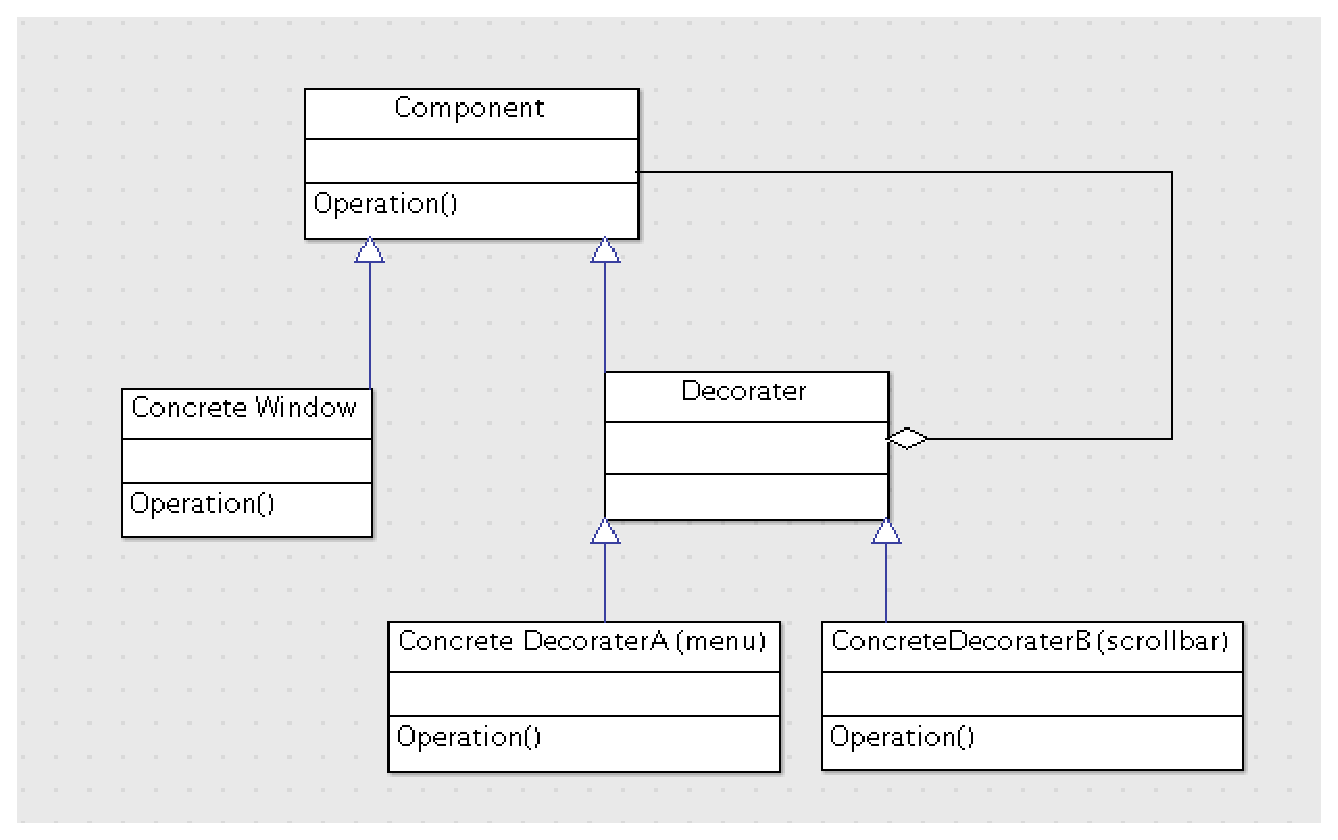
\includegraphics[scale=0.7]{lec9-1}
\end{center}
\begin{itemize}
\item Class Component 
\begin{itemize}
\item Defines the interface operations objects will provide 
\end{itemize}
\item Concrete Component - Implements the interface 
\item Decorator - all components inherit from Decorator, which inherits from component. So, every decorator is a component and every decorator has a component. 
\end{itemize}
\newpage
\begin{ex} Pizza
\begin{center}
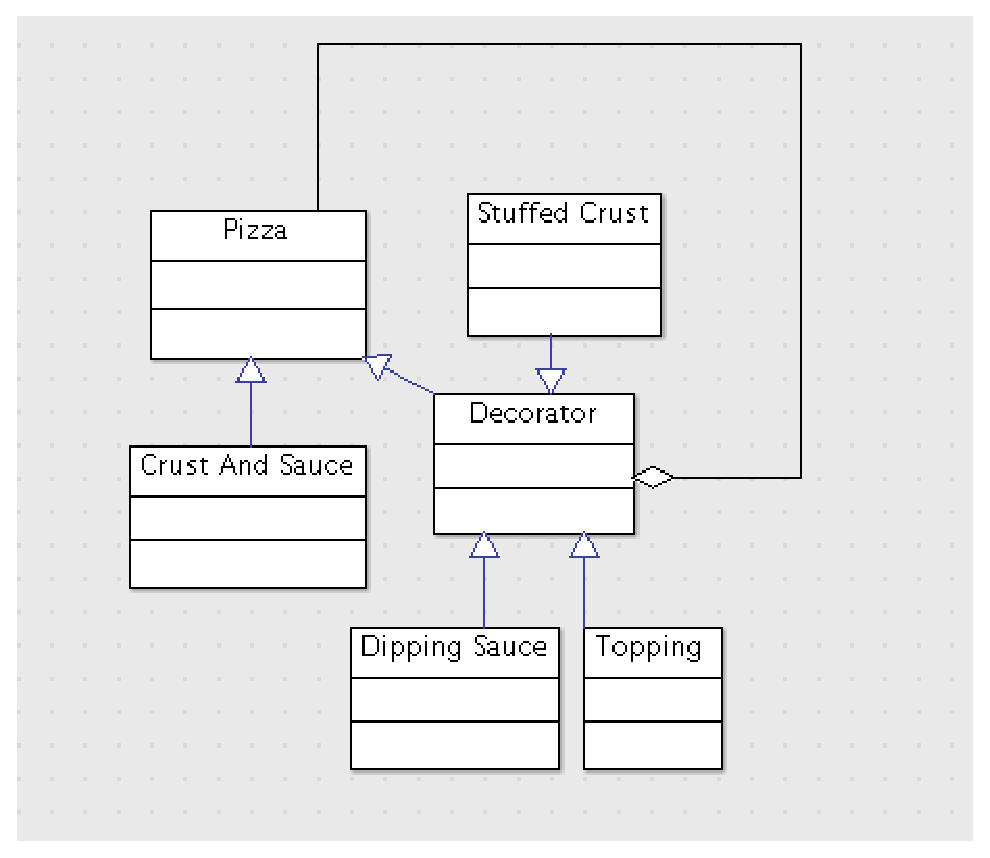
\includegraphics[scale=0.7]{lec9-3}
\end{center}
\begin{lstlisting}
Class Pizza {
	public :
		virtual float price () const =0;
		virtual string desc() const = 0;
		virtual ~pizza();
);

Class CrustAndSauce : public Pizza {
	public:
		float price() const override { return 5.99;}
		string desc() const override { return "Pizza";}
};

Class Decorator : public Pizza {
	protected : 
		Pizza component;
	public :
		Decorator (PIzza *p) : Component {p}{}
		virtual ~Decorator() {delete component;}
};

Class Topping : public Decorator {
		string theTopping;
	public :
		topping (string t, pizza *p) : Decorator {p}, theTopping{t}{}
		float price () const override {
			return component->price() + .75;
		}
		string desc() const override {
			return component->desc() + " with " + theTopping;
		}
};

int main () {
	Pizza *p1 = new CrustandSauce;
	p1 = new Topping ("Cheese", p1);
	p1 = new Topping ("Cheese", p1);
	
	cout << p1->desc() << p1->price();
	
	delete p1;
}
\end{lstlisting}
\end{ex}

\section{Inheritance and copy/move}
Consider : 
\begin{lstlisting}
Class Book {
	//Defines copy/move
};

Class Text : public Book {
	//Does not define copy/move 
};

Text t {"Algoithms". "CLRS", 500. "CS"};
Text tz = t; // No copy Ctor in Text 
\end{lstlisting}

There is no copy constructor so what happens is 
\begin{itemize}
\item Book's copy constructor is called 
\item then goes field-by field  for the text part 
\end{itemize}

\textbf{Write your own operations : }
\begin{lstlisting}
Text::Text(const Text &other) : Book {other}, topic{other.topic} {}

Text &text:: Operator= (const Text &other) {
	Book::Operator=(other);
	topic = other.topic;
	return *this 
}

Text::Text(Text &&other) : Book{std::move(other)}, topic{std::move(other.topic)} {}

Text &Text::operator=(Text &&other) {
	Book::Operator=(std::move(other));
	topic = std::move(other.topic);
	return *this;
}

\end{lstlisting}
	
\textbf{Note :} even though other points to an rvalue, it is it self a lvaue. \verb|std::move| forces an lvalue to be treated as a rvalue, so that "move" versions of the operators can be called. 

In addition, these custom operators are equivalent to the default operations, so they do not need to be defined. 
 \newpage
\textbf{Now Consider:}
\begin{lstlisting}
Text t1 { ... }, t2 {...} ;
Book *p1 = &t1, *p2 = &t2;
*p1 = *p2; // What happens?
\end{lstlisting}

When assigning a book point to a book pointer, we get a concept called \textbf{Partial Assignment}, as it only copies the book portion of the object. 
To fix this, we can set \verb|operator=| to be virtual .

\begin{lstlisting}
Class Book {
	public :
		virtual Book &operator=(const Book &other) ;
};

Class Text : Public Book {
	...
	public 
		Text &operator=(const Book  &other) override;
};
\end{lstlisting}

Different return types for virtual functions are ok (as long as you return a subclass reference/pointer), but different parameters must be the same or its not an override/compile and violates is-a. As a result, copying a book to a text in the example above, is technically legal, but can be a program breaking.

\textbf{Recommendation :} All superclasses should be abstract. 

\textbf{Rewrite Book Hierarchy :}

\begin{lstlisting}
Class AbstractBook{
		string title, author;
		int numPages;
	protected:
		AbstractBook &operator=(const AbstractBook &other);
	public :
		...
};

Class NormalBook : public AbstractBook {
	...
	public :
		...
		NormalBook &operator =(const NormalBook &other) {
			AbstractBook::operator(other);
			return *this;
		}
};
\end{lstlisting}

Now with the partial assignment example, assignment will be prevented for use by the base class. As a result, if partial assignment is done with this implementation, the application will not compile. 

\section{Factory Method Pattern}

Factory Method pattern lets a class defer instantiation to subclasses

\begin{ex} Basic Video Game -
A video game is created with 2 kinds of enemies (turtles and bullets), but bullets become more frequent later in the game.

\begin{center}
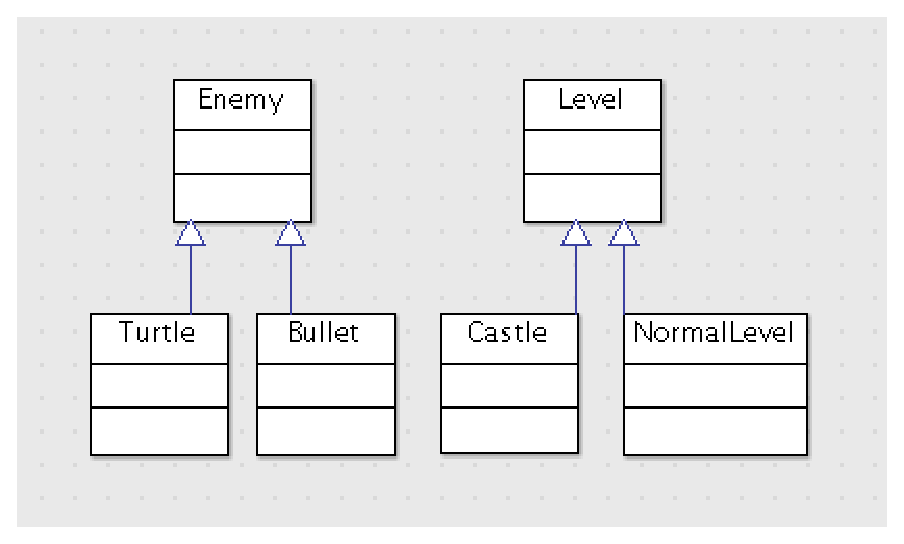
\includegraphics[scale=0.7]{lec9-2}
\end{center}

\begin{lstlisting}
Class Level {
		...
	public :
		virtual Enemy *createEnemy() = 0;
};

Class NormalLevel : pubic Level {
	public : 
		Enemy *createEnemy () override { /* create turtles */ }
};

Class Castle : public Level {
	public : 
		Enemy *createEnemy() override {/* mostly bullets */}
};

Level *l = new NormalLevel;
Enemy *e = l->createEnemy;

\end{lstlisting}
\end{ex}

\section{Template Method Pattern}
The template method pattern is used in any siutuition when you want subclasses to override superclass behaviour, but some aspects must remain the same. 

\begin{ex} There are red turtles and green turtles. 

\begin{lstlisting}
Class Turtle {
	public : 
		void draw () {
			drawHead();
			drawShell();
			drawFeet();
		}
	private : 
		void drawHead();
		void drawFeet();
		virtual void drawShell() = 0;
};

Class RedTurtle : public Turtle {
		void drawShell() override {/* draw red shell */}
};

Class GreenTurtle : public Turtle {
		void drawShell () override { /*draw green shell */}
};
\end{lstlisting}
\begin{itemize}
\item Most of the functions are defined an cannot, be overridden, but the functions listed as virtual allow for certain functionality to be modified. In the given example, sub classes can only change how the shell is drawn while everything else is already defined.
\end{itemize}
\end{ex}

\subsection{Extension : The Non-Virtual Interface (NVI) Idiom}
\begin{itemize}
\item A public virtual method is really two things :
\begin{itemize}
\item An interface to the client, which indicates provided behaviour, with pre/post conditions
\item An interface to subclasses, which has a hook to insert specialized behaviour.
\end{itemize}
\end{itemize}

It is hard to separate, these ideas if they are tied to the same function. 

The NVI idiom says : all public methods should be non-virtual and all virtual methods should be private or atleast protected, with the exception of the destructor. 

\begin{ex} Digital Media 
\begin{lstlisting}
// Without NVI
Class DigitalMedia {
	public : 
		virtual void play () = 0 ;
};

//With NVI
Class DigitalMedia {
	pubic :
		void play() { doPlay(); }
	private :
		virtual void doPlay () = 0; 
};
\end{lstlisting}
\end{ex}

This generalizes template method, by putting every virtual function call inside a template method.

\section{STL Map}

\begin{ex} "arrays" that map string to int
\begin{lstlisting}
#include <map>

//Creating a map
map<string, int> m;

//Add Values
m["abc"] = 1;
m["def"] = 4

//Printing
cout << m["ghi"]; // if key is not present, it is inserted with a default constructed value. 
cout << m["abc"]; //1

//Delete entry 
m.erase("abc");

//Check if a key exists 
if (m.count("abc") == 	1) { ... } 

//Iterating over a map -> sorted in order
for (auto &p : m){
	cout << p.first << " " << p.second << endl; //p's type is std::pair<string, int>
}
\end{lstlisting}
\end{ex}



\end{document}

\begin{ex} Decorator Pattern
\begin{lstlisting}

\end{lstlisting}
\end{ex}



\end{document}









